\documentclass[conference]{IEEEtran}
\usepackage{amsmath,amssymb,graphicx,float,booktabs,cite,hyperref,listings,enumitem,url}
\usepackage[T1]{fontenc}
\usepackage[table]{xcolor}

\lstdefinelanguage{Solidity}{
  keywords={pragma,solidity,contract,function,public,internal,view,returns,require,emit,event,struct,mapping,address,bool,uint256,bytes32,memory,if,else,return},
  keywordstyle=\color{blue}\bfseries,sensitive=true,
  comment=[l]{//},commentstyle=\color{green!60!black},
  stringstyle=\color{red!70!black},morestring=[b]"
}
\lstset{basicstyle=\ttfamily\scriptsize,breaklines=true,frame=single,numbers=left,numberstyle=\tiny\color{gray},showstringspaces=false,tabsize=2}
\hypersetup{colorlinks=true,linkcolor=black,citecolor=black,urlcolor=blue}

\begin{document}

\title{Bharat E-Vote: A Blockchain-Based Electronic Voting System with Commitment-Based Privacy and Multi-Layered Security}

\author{
\IEEEauthorblockN{Aditya Bhoir}
\IEEEauthorblockA{\textit{Department of Computer Engineering} \\
\textit{PES Modern College of Engineering}\\
Pune, India \\
aditya\_bhoir\_comp@moderncoe.edu.in}
\and
\IEEEauthorblockN{Omkar Ingle}
\IEEEauthorblockA{\textit{Department of Computer Engineering} \\
\textit{PES Modern College of Engineering}\\
Pune, India \\
omkar\_ingle\_comp@moderncoe.edu.in}
\and
\IEEEauthorblockN{Aftab Pathan}
\IEEEauthorblockA{\textit{Department of Computer Engineering} \\
\textit{PES Modern College of Engineering}\\
Pune, India \\
aftab\_pathan\_comp@moderncoe.edu.in}
\and
\IEEEauthorblockN{Abhishek Shinde}
\IEEEauthorblockA{\textit{Department of Computer Engineering} \\
\textit{PES Modern College of Engineering}\\
Pune, India \\
abhishek\_shinde\_comp@moderncoe.edu.in}
\and
\IEEEauthorblockN{Aryan Shinde}
\IEEEauthorblockA{\textit{Department of Computer Engineering} \\
\textit{PES Modern College of Engineering}\\
Pune, India \\
aryan\_shinde\_comp@moderncoe.edu.in}
\and
\IEEEauthorblockN{Dr.\ B.\ D.\ Phulpagar}
\IEEEauthorblockA{\textit{Department of Computer Engineering} \\
\textit{PES Modern College of Engineering}\\
Pune, India \\
bdphulpagar@moderncoe.edu.in}
}

\maketitle

% ===== ABSTRACT =====
\begin{abstract}
Traditional electronic voting systems rely on centralized trust, lack independent verifiability, and offer limited ballot privacy. This paper presents \textbf{Bharat E-Vote}, a decentralized electronic voting platform built on Ethereum smart contracts with a hash-based commitment scheme for vote privacy and a seven-layer defense-in-depth security architecture. Votes are recorded as immutable blockchain state transitions. A commitment scheme based on finite-field arithmetic hides voter choices, while a simplified proof-of-knowledge protocol provides a structural framework for on-chain verification (with limitations discussed in Section~IV-B). The security architecture combines bot protection with rate limiting, OTP-based multi-factor authentication with httpOnly cookie-based JWT transport, keystroke dynamics anomaly detection, smart contract role-based access control, HTTP parameter pollution prevention, and HTTP security header enforcement. An ERC-2771 meta-transaction forwarder~\cite{openzeppelin2024} enables gasless voting. The system was validated through 49 automated smart contract tests and 9 backend API integration tests (100\% pass rate across 58 total tests). Performance benchmarks show vote inclusion in blocks within 12--18 seconds on Ethereum Sepolia testnet (with probabilistic finality at approximately 12 minutes), and API response times below 150ms. We present an honest assessment of the system's limitations, including the proof-of-concept nature of the privacy module and the trust assumptions inherent in the architecture.
\end{abstract}

\begin{IEEEkeywords}
Blockchain, Ethereum, Smart Contracts, Commitment Schemes, Multi-Factor Authentication, Keystroke Dynamics, ERC-2771, Defense-in-Depth, Electronic Voting
\end{IEEEkeywords}

% ===== I. INTRODUCTION =====
\section{Introduction}

The integrity of democratic governance depends on trustworthy elections. Electronic voting offers improved efficiency but introduces significant vulnerabilities: centralized databases as single points of failure, opaque tallying software, and network-level threats~\cite{kshetri2018}. India's EVM infrastructure serves approximately 960 million voters~\cite{eci2024} but operates as closed-source devices where counting firmware cannot be publicly audited.

Existing blockchain-based voting proposals address immutability but frequently neglect ballot privacy, multi-factor authentication, or usability for non-technical voters. This paper presents \textbf{Bharat E-Vote}, which contributes:

\begin{itemize}[leftmargin=*]
    \item \textbf{On-Chain Verifiability:} Every vote is an Ethereum blockchain transaction enforced by a Solidity smart contract, enabling independent result recomputation.
    \item \textbf{Commitment-Based Privacy:} A hash-based commitment module hides vote choices on-chain, with a simplified proof-of-knowledge protocol for verification. We explicitly characterize this as a proof-of-concept and discuss its limitations relative to algebraically homomorphic Pedersen commitments.
    \item \textbf{Defense-in-Depth:} Seven security layers ensure no single-point compromise defeats the system.
    \item \textbf{Gasless Voting:} ERC-2771 meta-transactions remove the cryptocurrency prerequisite, though we acknowledge the censorship risk of centralized relayers.
    \item \textbf{Partial Coercion Mitigation:} A re-voting mechanism (up to 3 re-votes) raises the cost of coercion, though it does not achieve receipt-freeness as defined by Juels et al.~\cite{juels2005}.
    \item \textbf{Honest Limitations Analysis:} A dedicated section enumerates trust assumptions and architectural constraints, including relayer censorship, wallet linkability, and database metadata exposure.
\end{itemize}

% ===== II. RELATED WORK =====
\section{Related Work}

Hardwick et al.~\cite{hardwick2018} propose a blockchain-based e-voting protocol using Ethereum as a transparent ballot box, but evaluate it only as a small-scale proof-of-concept with limited scalability analysis. The protocol lacks multi-factor authentication and gasless transaction support. Hj{\'a}lmarsson et al.~\cite{hjalmarsson2018} demonstrate a Solidity-based voting contract but evaluate it only on a local Ganache network with four simulated voters, leaving open the question of whether their gas cost analysis holds under real network congestion. Their system does not address ballot secrecy or re-voting mechanisms. Kshetri and Voas~\cite{kshetri2018} discuss the potential and challenges of blockchain-enabled e-voting, noting that while blockchain provides transparency and immutability, scalability and gas costs remain critical barriers for large-scale elections.

Ometov et al.~\cite{ometov2018} survey multi-factor authentication methods spanning knowledge, possession, and inherence factors, but their analysis draws primarily from enterprise and mobile banking deployments rather than election-specific use cases where adversarial models differ substantially. Maheshwary et al.~\cite{maheshwary2022} provide a systematic literature review of keystroke dynamics models, identifying six design patterns for typing-based authentication and reporting accuracy rates of 90--95\% across major studies.

Farooq et al.~\cite{farooq2022} propose a framework for transparent voting using blockchain, with smart contracts for automated vote management, but do not address voter privacy through cryptographic commitments. Helios~\cite{adida2008} provides web-based auditable voting but lacks blockchain immutability. Juels et al.~\cite{juels2005} formalize coercion resistance through receipt-freeness---the inability to prove to a coercer how one voted---which remains an open challenge for practical systems.

\begin{table}[htbp]
\centering
\caption{Comparison with Existing Voting Systems}
\label{tab:comparison}
\renewcommand{\arraystretch}{1.1}
\scriptsize
\begin{tabular}{|p{2cm}|c|c|c|c|}
\hline
\textbf{Feature} & \textbf{EVM} & \textbf{Helios} & \textbf{Hardwick} & \textbf{Ours} \\
\hline
Decentralized & No & Partial & Yes & Yes \\
\hline
Voter Verifiable & No & Yes & Partial & Yes \\
\hline
Ballot Privacy & Yes & Yes & Partial & Partial$^*$ \\
\hline
Tamper Proof & Partial & Partial & Partial & Partial$^\S$ \\
\hline
Coercion Resist. & No & No & No & Partial$^\dagger$ \\
\hline
Multi-Factor Auth & No & No & No & Yes \\
\hline
Gasless Voting & N/A & N/A & No & Yes$^\ddagger$ \\
\hline
\end{tabular}

\vspace{2pt}
\scriptsize{$^*$Hash-based commitment (proof-of-concept); does not achieve algebraic Pedersen hiding.\\
$^\dagger$Re-voting mitigation; does not achieve receipt-freeness~\cite{juels2005}.\\
$^\ddagger$Via centralized relayer with censorship risk (see Section~VII-D).\\
$^\S$Standard mode is tamper-proof on-chain; ZKP mode lacks on-chain tallying; off-chain DB and relayer introduce trust assumptions.}
\end{table}

\begin{figure}[htbp]
\centering
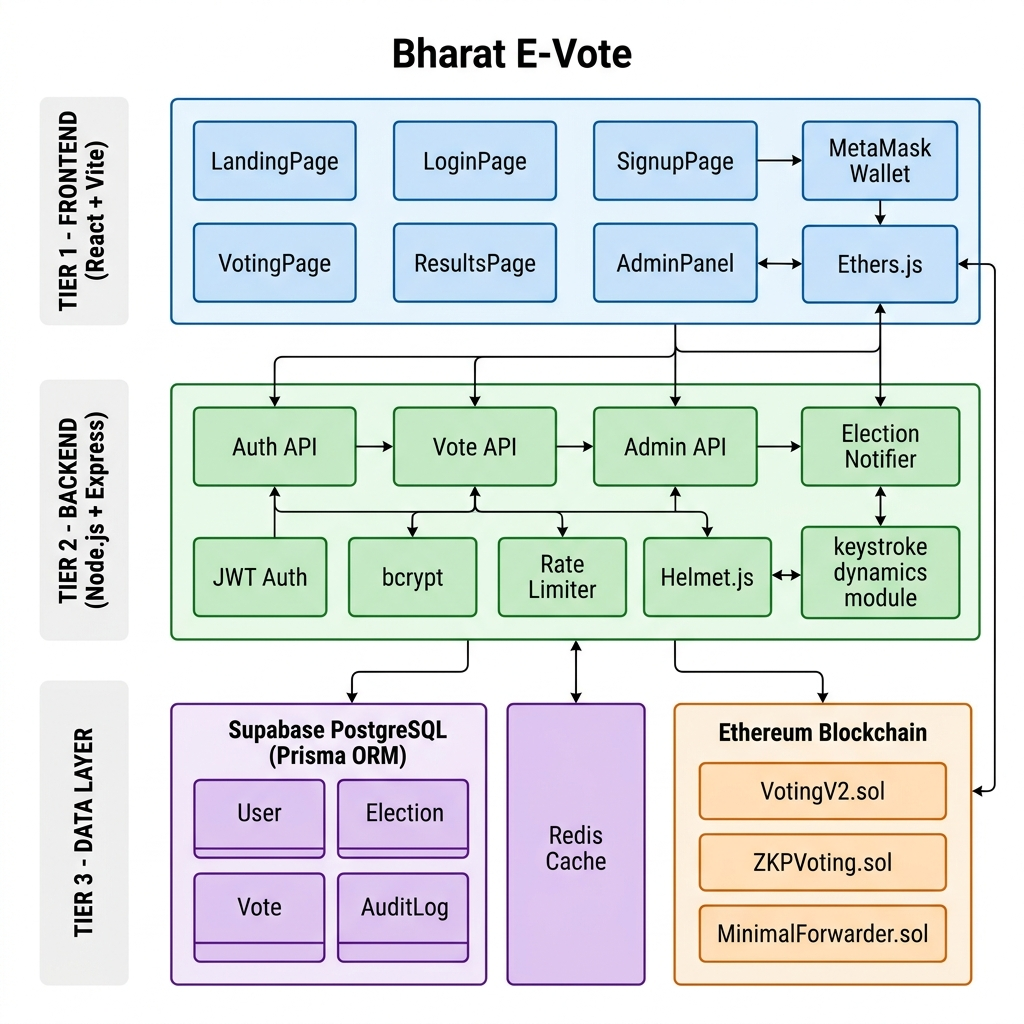
\includegraphics[width=0.48\textwidth]{images/System_Architecture_Diagram.jpeg}
\caption{System Architecture Diagram --- Three-tier decentralized architecture with React frontend, Node.js backend, and Ethereum blockchain as the final trust boundary.}
\label{fig:arch}
\end{figure}

\begin{figure}[htbp]
\vspace{1em}
\centering
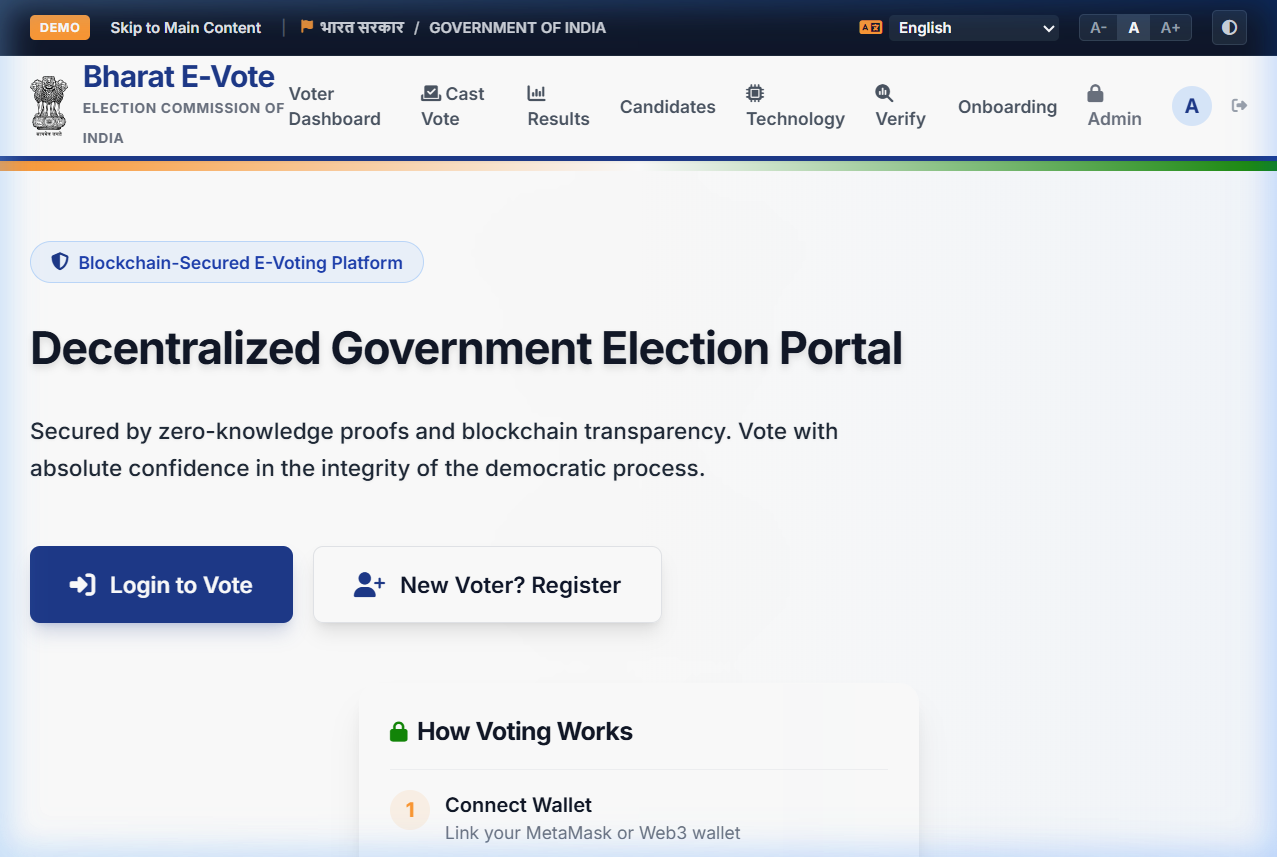
\includegraphics[width=0.48\textwidth]{images/landing_page.jpeg}
\caption{Bharat E-Vote Landing Page --- National portal interface with citizen services grid and biometric verification prompt.}
\label{fig:landing}
\end{figure}

% ===== III. SYSTEM ARCHITECTURE =====
\section{System Architecture}

As illustrated in Fig.~\ref{fig:arch}, Bharat E-Vote uses a three-tier architecture: React 19/Vite frontend (accessible via the national portal, Fig.~\ref{fig:landing}), Node.js/Express~5 backend, and Ethereum blockchain. The blockchain smart contract is the final trust boundary for vote integrity, though off-chain components introduce additional trust assumptions (Section~VIII).

\subsection{Smart Contract Layer}
Two contracts handle voting through mode-based separation:
\begin{itemize}[leftmargin=*]
    \item \textbf{VotingV2.sol} (standard mode): Candidate management, voter authorization, vote casting with re-voting, constituency matching, and on-chain tallying. When \texttt{zkpEnabled=true}, this contract's \texttt{vote()} function reverts, forcing votes through the privacy contract.
    \item \textbf{ZKPVoting.sol} (privacy mode): Commitment-based voting with nullifier-based double-vote prevention and a simplified proof-of-knowledge verification. \textbf{Important:} This contract stores commitments but does not perform on-chain tallying---vote counts are not incremented per-candidate. The privacy module securely records encrypted votes but lacks the cryptographic mechanisms to count them automatically. Result determination in ZKP mode would require either homomorphic tallying over commitments (not possible with our SHA-256-wrapped scheme) or a trusted off-chain tally, which reintroduces the centralization problem. This tallying gap is a known limitation (Section~VII-D).
\end{itemize}
A third contract, \textbf{MinimalForwarder.sol}~\cite{openzeppelin2024}, implements ERC-2771 meta-transactions for gasless voting.

\subsection{Data Flow}
(1) Voter authenticates via backend MFA; (2) connects MetaMask wallet and accesses the dashboard (Fig.~\ref{fig:dashboard}); (3) frontend invokes the appropriate contract via Ethers.js using the proctored interface (Fig.~\ref{fig:voting}); (4) smart contract validates authorization and records the vote; (5) results are read from on-chain state and displayed publicly (Fig.~\ref{fig:results}).

% ===== IV. CRYPTOGRAPHIC PROTOCOLS =====
\section{Commitment and Verification Protocols}

\subsection{Hash-Based Commitment Scheme}

The system implements a commitment scheme using finite-field exponentiation with parameters derived from the secp256k1 scalar field, followed by a SHA-256 hash. Following Pedersen~\cite{pedersen1991}, let $p$ be the secp256k1 group order. Let $g$ and $h$ be large integers derived from the x-coordinates of two secp256k1 curve points; these are treated as elements of $\mathbb{Z}_p^*$, not as elliptic curve points.

\textbf{Commitment Phase (browser-side):}
\begin{enumerate}[leftmargin=*]
    \item Compute $C_{\text{raw}} = g^v \cdot h^r \bmod p$ where $v$ is the candidate ID and $r$ is a 256-bit random blinding factor.
    \item Compute $C = \text{SHA-256}(C_{\text{raw}})$ --- the published on-chain commitment.
\end{enumerate}

\textbf{Distinction from Standard Pedersen Commitments:} A standard Pedersen commitment~\cite{pedersen1991} is defined as $C = g^v \cdot h^r \bmod p$ \emph{without} the hash wrapper. The algebraic structure preserves the \emph{homomorphic property} ($C_1 \cdot C_2 = g^{v_1+v_2} \cdot h^{r_1+r_2}$), enabling verifiable tallying without decrypting individual votes. Our SHA-256 wrapper destroys this property, converting the scheme into a standard hash commitment. While the commitment remains \emph{computationally hiding} (SHA-256 preimage resistance) and \emph{computationally binding} (collision resistance), it loses the algebraic structure that enables efficient zero-knowledge proofs over committed values. We identify migration to proper elliptic curve Pedersen commitments ($C = v \cdot G + r \cdot H$ where $G$, $H$ are curve points) as critical future work.

\subsection{Simplified Proof-of-Knowledge Protocol}

The on-chain verifier implements a simplified check rather than a full Schnorr sigma protocol~\cite{schnorr1991}. Voters can independently verify their ballot using the interface shown in Fig.~\ref{fig:zkp}. The prover (browser) computes:
\begin{align}
e &= H(C, N, k_v, k_r, n) \bmod p \\
s_v &= (k_v - e \cdot v) \bmod p \\
s_r &= (k_r - e \cdot r) \bmod p
\end{align}
where $k_v, k_r$ are random nonces and $n$ is the candidate count.

The on-chain verifier checks:
\[ H(C, N, s_v, s_r, n) \bmod p \stackrel{?}{=} e \]

\textbf{Limitation (Critical):} In a correct Schnorr sigma protocol for a Pedersen commitment, the verifier must reconstruct the announcement: $R' = g^{s_v} \cdot h^{s_r} \cdot C^e \bmod p$, then verify $H(C, N, R', n) = e$. Our simplified verifier hashes the responses directly without algebraic reconstruction, meaning a prover can manufacture a passing proof by computing $e = H(C, N, s_v, s_r, n)$ for arbitrary $s_v, s_r$. \textbf{The current implementation does not constitute a zero-knowledge proof.} It serves as a structural placeholder demonstrating the integration pattern (client-side proof generation $\rightarrow$ on-chain verification $\rightarrow$ nullifier tracking). Implementing a correct sigma protocol with on-chain modular exponentiation (feasible but gas-intensive) is identified as essential future work.

\subsection{Nullifier-Based Double-Vote Prevention}
This component functions correctly: $N = H(\text{voterSecret}, \text{electionId})$ is deterministic per voter per election. The mapping \texttt{nullifierUsed[N]} prevents reuse. Identity commitments $IC = H(\text{voterSecret})$ are registered on-chain by the admin. \textbf{Privacy caveat:} In the current implementation, the admin receives the voter's secret to compute $IC$, enabling the admin to derive the voter's nullifier and link it to their identity. This breaks the unlinkability guarantee of the nullifier scheme (see Section~VII-D). The correct approach---having voters compute and submit their own $IC$ with the admin only whitelisting it---is identified as future work.

\subsection{Standard Mode Privacy Limitations \& Event Obfuscation}
The \texttt{VoteCast} event emits $\text{keccak256}(\text{candidateId}, \text{msgSender}, \text{timestamp}, \text{secretSalt})$, where \texttt{secretSalt} is a 256-bit random value generated off-chain by the voter's browser. The inclusion of a secret off-chain salt makes brute-force enumeration of the \emph{event log} computationally infeasible. \textbf{However, this provides only superficial obfuscation in standard mode:} to support the re-voting mechanism, the \texttt{Voter} struct must store the \texttt{lastCandidateId} on-chain to decrement previous votes. This exposes the vote choice in the plaintext blockchain state, rendering the event obfuscation cosmetic for anyone querying the state trie directly. Full ballot privacy is only achievable through the ZKP mode.

% ===== V. SECURITY ARCHITECTURE =====
\section{Seven-Layer Defense-in-Depth Security}

The security architecture comprises seven functionally distinct layers. Bot protection and rate limiting, though implemented via three distinct technologies (Cloudflare Turnstile, express-rate-limit, Upstash Redis), are grouped as a single perimeter layer as they implement the same control class.

\begin{table}[htbp]
\centering
\caption{Seven-Layer Defence-in-Depth Architecture}
\label{tab:security}
\renewcommand{\arraystretch}{1.15}
\scriptsize
\begin{tabular}{|c|p{2.2cm}|p{4.3cm}|}
\hline
\textbf{L} & \textbf{Technology} & \textbf{Purpose} \\
\hline
1 & Cloudflare + express-rate-limit + Redis & Perimeter defense: bot blocking, per-IP throttling, distributed sliding-window rate limiting \\
\hline
2 & Password + OTP + httpOnly JWT & Multi-factor identity verification with httpOnly, Secure, SameSite=Strict cookie-based JWT transport; single-active-session enforcement; XSS-resistant token storage \\
\hline
3 & Keystroke Dynamics & Behavioural anomaly \emph{detection} (alerts admin; does not block session)$^*$ \\
\hline
4 & Smart Contract RBAC & On-chain role enforcement; admin blocked from voting \\
\hline
5 & Express Middleware & Payload size limiting (10KB), XSS input sanitization, HTTP Parameter Pollution (hpp) prevention \\
\hline
6 & Helmet.js & CSP, HSTS, X-Frame-Options, X-Content-Type-Options \\
\hline
7 & Cookie Security & httpOnly + Secure + SameSite=Strict cookie flags; eliminates localStorage XSS attack vector for JWT tokens \\
\hline
\end{tabular}

\vspace{2pt}
\scriptsize{$^*$Keystroke dynamics acts as an administrative audit tool and \emph{monitoring} layer, rather than a deterministic access blocker. It flags behavioural anomalies without terminating sessions. See Section~VIII.}
\end{table}

\subsection{Multi-Factor Authentication}
Two-step MFA: Step~1 verifies password via \texttt{bcrypt} (cost factor 12), generates a 6-digit OTP (hashed, 5-minute expiry); Step~2 verifies OTP and issues JWT (20-minute expiry) delivered as an \texttt{httpOnly}, \texttt{Secure}, \texttt{SameSite=Strict} cookie, with single-active-session enforcement via Redis. The httpOnly cookie transport eliminates the localStorage-based XSS vulnerability present in earlier versions where JavaScript code could extract the JWT token.

\subsection{Partial Coercion Mitigation}
The re-voting mechanism allows up to 3 vote changes (\texttt{MAX\_REVOTES=3}), atomically adjusting candidate counts. This raises the cost of coercion but \textbf{does not achieve receipt-freeness}~\cite{juels2005}: a coercer controlling the voter for the final voting attempt can ensure the coerced vote is counted. We characterize this as \emph{partial coercion mitigation}, not coercion resistance.

% ===== VI. IMPLEMENTATION =====
\section{Implementation}

\subsection{Technology Stack}
Solidity version 0.8.19 (smart contracts), Hardhat (testing), Ethers.js v6 (blockchain interaction), Node.js/Express~5 (backend), Prisma ORM over Supabase PostgreSQL (16 models), React 19/Vite (frontend), MetaMask (wallet).

\subsection{Vote Function Design}
The \texttt{vote()} function follows the Checks-Effects-Interactions pattern:

\begin{lstlisting}[language=Solidity]
function vote(uint256 _candidateId,
              uint256 _secretSalt) public {
  require(!zkpEnabled, "Use ZKP contract");
  require(_msgSender() != admin);
  require(voters[sender].isAuthorized);
  // Re-vote: decrement old candidate
  if (voters[sender].hasVoted) {
    candidates[voters[sender].lastCandidateId]
      .voteCount--;
  }
  candidates[_candidateId].voteCount++;
  voters[sender].hasVoted = true;
  emit VoteCast(
    keccak256(abi.encodePacked(
      _candidateId, _msgSender(),
      block.timestamp, _secretSalt)),
    block.timestamp, voter.voteVersion);
}
\end{lstlisting}

\subsection{Gas Cost Analysis}
\begin{table}[htbp]
\centering
\caption{Gas Cost Per Operation (Sepolia Testnet)}
\label{tab:gas}
\renewcommand{\arraystretch}{1.15}
\scriptsize
\begin{tabular}{|p{3cm}|r|r|}
\hline
\textbf{Operation} & \textbf{Gas Units} & \textbf{Est.\ Cost}$^*$ \\
\hline
\texttt{vote()} (first vote) & $\sim$85,000 & \$2.13 \\
\hline
\texttt{vote()} (re-vote) & $\sim$95,000 & \$2.38 \\
\hline
\texttt{authorizeVoter()} & $\sim$65,000 & \$1.63 \\
\hline
\texttt{submitEncryptedVote()} & $\sim$120,000 & \$3.00 \\
\hline
\texttt{addCandidate()} & $\sim$110,000 & \$2.75 \\
\hline
\end{tabular}

\vspace{2pt}
\scriptsize{$^*$At 10 gwei gas price and ETH=\$2,500. Mainnet costs vary significantly. At 50 gwei, costs are 5x higher. For 960M voters, total gas cost for \texttt{vote()} plus \texttt{authorizeVoter()} would be approximately \$3.6 Billion (\$2.13+\$1.63 per voter at 10 gwei, scaling linearly with gas price), making Layer-2 deployment absolutely essential for national scale.}
\end{table}

\begin{figure}[htbp]
\centering
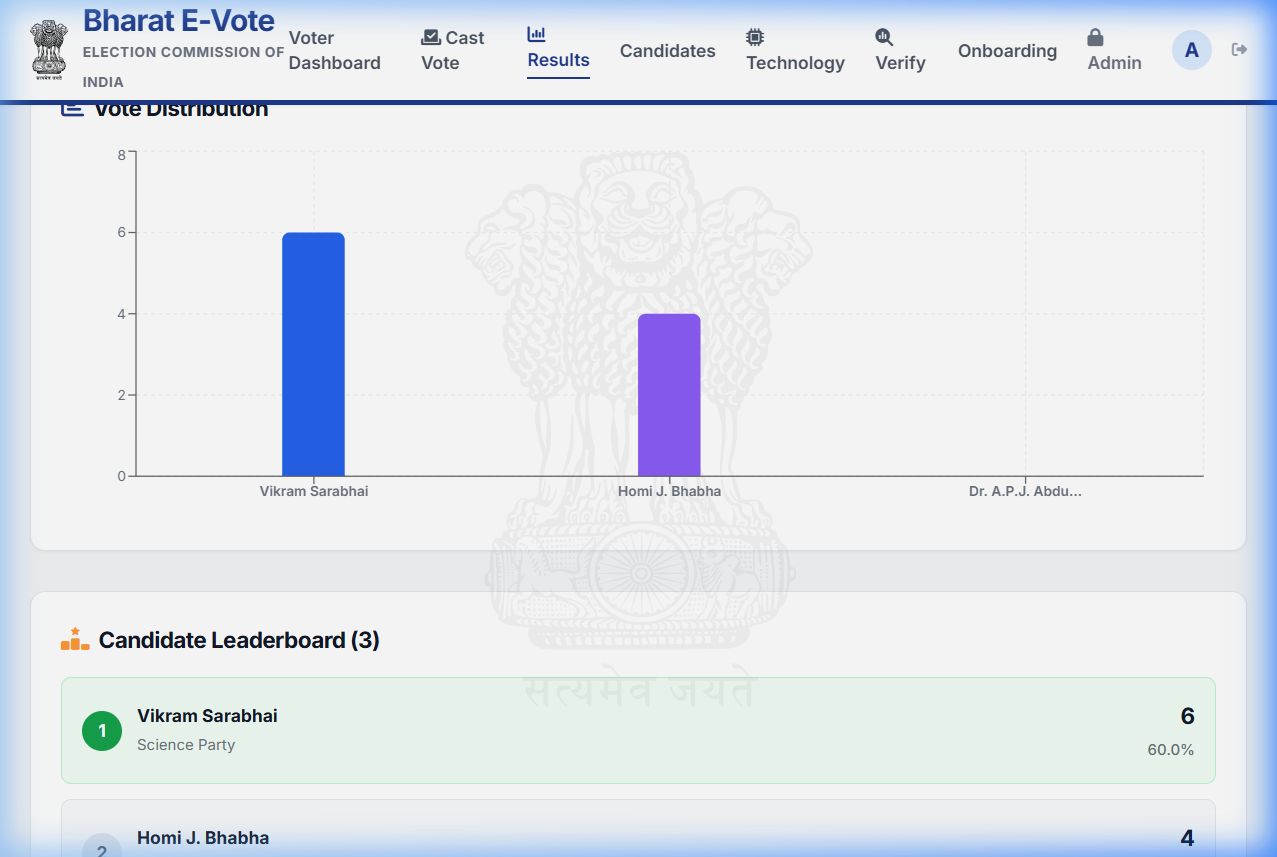
\includegraphics[width=0.48\textwidth]{images/proctored_voting.jpeg}
\caption{Proctored Voting Interface --- Candidate ballot cards with constituency filtering and re-vote support. The voter selects a candidate and the vote is submitted as a blockchain transaction.}
\label{fig:voting}
\end{figure}

\begin{figure}[htbp]
\centering
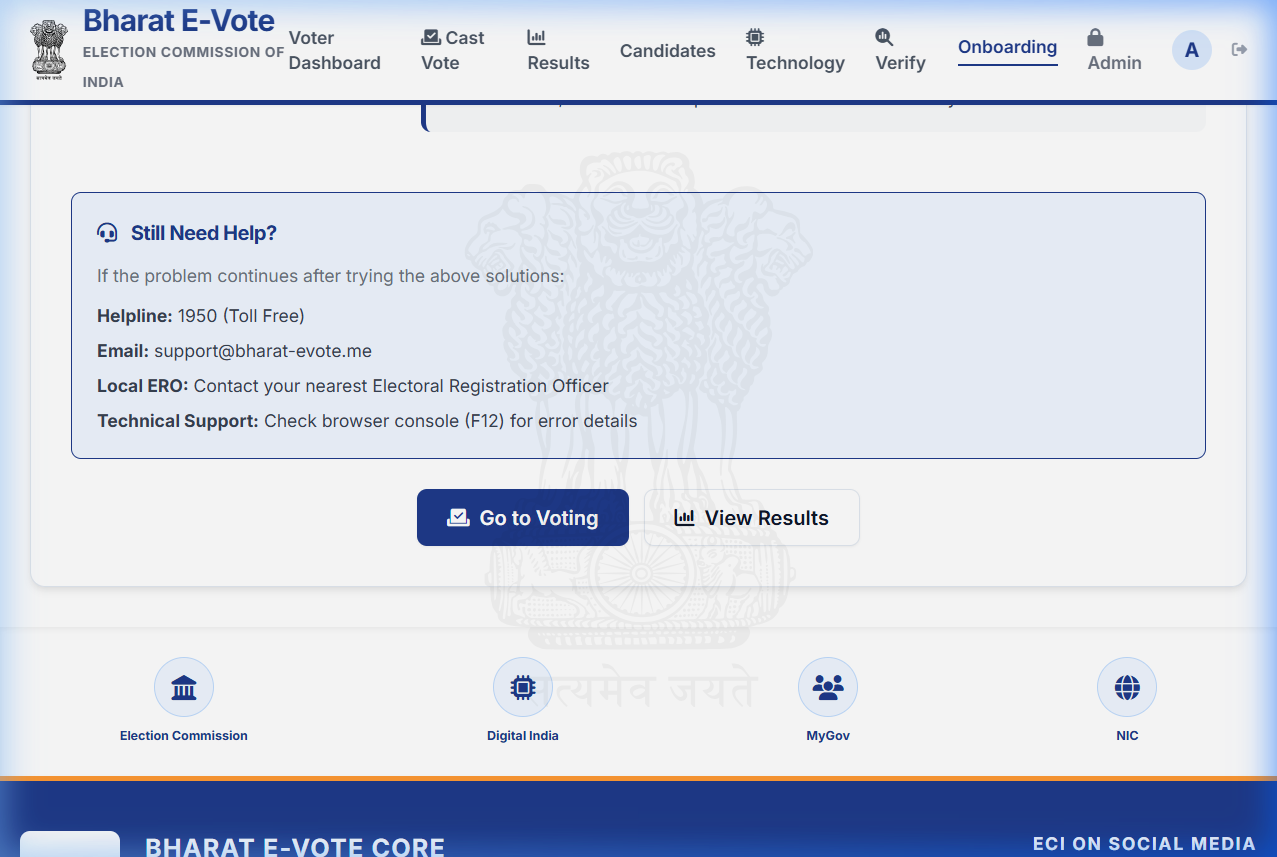
\includegraphics[width=0.48\textwidth]{images/voter_dashboard.jpeg}
\caption{Voter Dashboard --- Authenticated voter home page showing election status, profile information, and navigation to voting and results pages.}
\label{fig:dashboard}
\end{figure}

\begin{figure}[htbp]
\centering
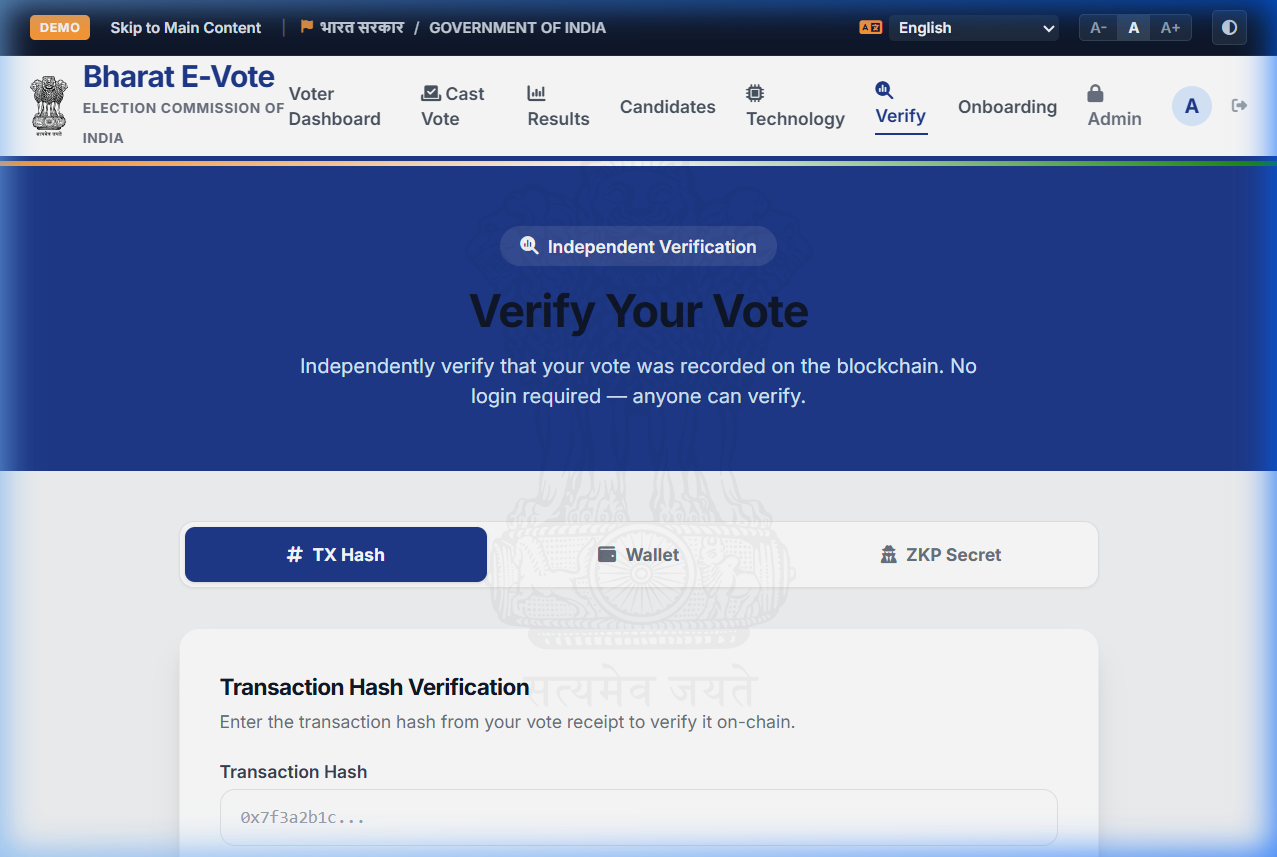
\includegraphics[width=0.48\textwidth]{images/zkp_verification.jpeg}
\caption{ZKP Vote Verification --- On-chain vote commitment verification page where voters can verify their encrypted ballot using the nullifier hash.}
\label{fig:zkp}
\end{figure}

% ===== VII. EXPERIMENTAL RESULTS =====
\section{Experimental Results}

\subsection{Smart Contract Testing}
49 automated smart contract tests (Hardhat/Chai/Mocha) validated the following functional categories: deployment, access control, vote casting, re-voting, constituency matching, timeline enforcement, event privacy, nullifier enforcement, vote verifiability, ERC-2771 meta-transactions, IPFS metadata storage, and ZKP mode integration. VotingV2.sol: 11 tests; ZKPVoting.sol: 38 tests. All passed (100\% rate).

\subsection{Backend API Testing}
9 backend integration tests (Jest/Supertest) validated the REST API layer across three endpoint groups: authentication (4 tests covering registration validation, login flow, and credential verification), vote recording (4 tests covering authentication enforcement, transaction hash validation, and vote status queries), and cryptographic ballot privacy (3 tests covering ZKP status endpoints, commitment generation, and proof verification parameter validation). All passed (100\% rate).

\subsection{Performance}
\begin{table}[htbp]
\centering
\caption{Performance Results}
\label{tab:performance}
\renewcommand{\arraystretch}{1.15}
\scriptsize
\begin{tabular}{|p{2.5cm}|c|c|c|}
\hline
\textbf{Metric} & \textbf{Target} & \textbf{Achieved} & \textbf{Status} \\
\hline
Login Auth Time & $<$3s & 1.8s & Met \\
\hline
Block Inclusion (Sepolia) & $<$30s & 12--18s & Met \\
\hline
Finality (Sepolia)$^*$ & --- & $\sim$12 min & --- \\
\hline
Vote (Hardhat) & $<$2s & 0.8s & Met \\
\hline
API Read & $<$200ms & 85--150ms & Met \\
\hline
\end{tabular}

\vspace{2pt}
\scriptsize{$^*$Ethereum PoS achieves probabilistic finality after 2 epochs ($\sim$12 minutes). Block inclusion (12--18s) does not guarantee finality; reorganizations can occur before finalization. For election integrity, results should not be declared until finality is achieved for all vote transactions.}
\end{table}

\begin{figure}[htbp]
\centering
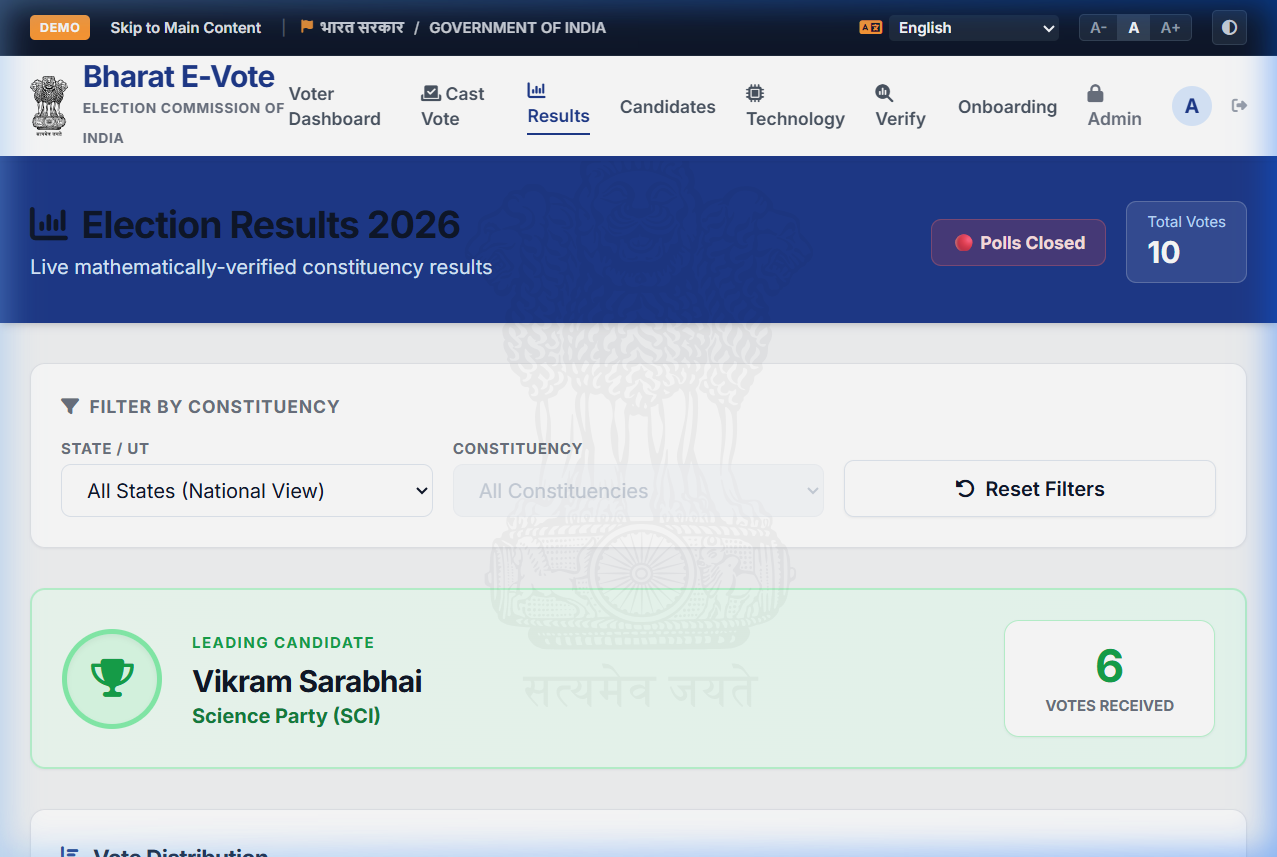
\includegraphics[width=0.48\textwidth]{images/election_results.jpeg}
\caption{Election Results --- Real-time vote counts read from the blockchain, rendered as bar charts and pie charts using Recharts.}
\label{fig:results}
\end{figure}


\subsection{Security Validation}
We performed STRIDE-based threat modeling and countermeasure mapping (not a formal security proof) across all six categories:

\begin{table}[htbp]
\centering
\caption{STRIDE-Based Threat Modeling}
\label{tab:stride}
\renewcommand{\arraystretch}{1.1}
\scriptsize
\begin{tabular}{|p{1.4cm}|p{1.5cm}|p{4.3cm}|}
\hline
\textbf{Category} & \textbf{Threat} & \textbf{Countermeasure} \\
\hline
Spoofing & Impersonation & MFA + single-session; keystroke anomaly alerts \\
\hline
Tampering & Vote manip. & Blockchain immutability + CEI pattern \\
\hline
Repudiation & Deny vote & On-chain receipt hash + audit logs \\
\hline
Info.\ Disc. & Vote reveal & Candidate ID excluded from struct; event obfuscation via secret salt (see Sec.~IV-D) \\
\hline
DoS & Flooding & Rate limiting + bot protection (Layer 1) \\
\hline
Elev.\ Priv. & Admin escal. & JWT verification + on-chain RBAC \\
\hline
\end{tabular}
\end{table}

% ===== VII-D. CONCLUSION, LIMITATIONS, AND FUTURE WORK =====
\section{Conclusion, Limitations, and Future Work}

\subsection{Summary}
This paper presented Bharat E-Vote, a blockchain-based voting platform that achieves on-chain verifiability and multi-layered security. The system was validated through 58 automated tests---49 smart contract tests and 9 backend API integration tests---achieving a 100\% pass rate, and met all performance targets.

\subsection{Limitations and Trust Assumptions}
We explicitly enumerate the system's limitations:

\begin{enumerate}[leftmargin=*]
    \item \textbf{Privacy Module is Proof-of-Concept:} The ZKP logic within \texttt{ZKPVoting.sol} uses a simulated Schnorr-like challenge mechanism rather than a true SNARK verifier (e.g., Circom). The module demonstrates the \emph{integration architecture} (client-side proof $\rightarrow$ on-chain verification $\rightarrow$ nullifier tracking) but does not provide cryptographically secure zero-knowledge guarantees.

    \item \textbf{Web2 Centralized Onboarding:} Voter eligibility relies on a centralized PostgreSQL database managed by administrators. In a fully decentralized architecture, this would be replaced by an On-Chain Decentralized Identity (DID) standard (e.g., Polygon ID).

    \item \textbf{ZKP Mode Has No Tallying Mechanism:} \texttt{ZKPVoting.sol} stores commitments but does not increment per-candidate vote counts. Result determination would require either homomorphic tallying or a trusted off-chain tally, reintroducing centralization.

    \item \textbf{ERC-2771 Relayer is a Trusted Party:} The centralized relayer can censor votes by refusing to forward transactions, with no on-chain accountability.

    \item \textbf{MetaMask Wallet Linkability:} Transaction timing and wallet history can deanonymize voters through network analysis.

    \item \textbf{No Receipt-Freeness:} The re-voting mechanism does not prevent a coercer from controlling the final vote attempt~\cite{juels2005}.

    \item \textbf{Block Inclusion vs.\ Finality:} Ethereum PoS achieves finality after $\sim$12 minutes; votes may be reorganized before finalization.

    \item \textbf{Smart Contract Immutability:} Mid-election bugs cannot be patched without introducing a trusted upgrade authority.
\end{enumerate}

\subsection{Future Work}
\begin{enumerate}[leftmargin=*]
    \item \textbf{Correct ZKP Implementation:} Replace the simplified verifier with a proper Schnorr sigma protocol including algebraic announcement reconstruction, and migrate to elliptic curve Pedersen commitments ($C = v \cdot G + r \cdot H$) to restore homomorphic properties and enable on-chain tallying.
    \item \textbf{Self-Sovereign Identity Commitments:} Have voters compute and submit their own $IC$, eliminating admin knowledge of voter secrets.
    \item \textbf{Layer-2 Scaling:} Deploy on Polygon zkEVM or Optimism to reduce gas costs by $\sim$100x.
    \item \textbf{Decentralized Relayer:} Replace the centralized meta-transaction relayer with OpenGSN.
    \item \textbf{Receipt-Freeness:} Investigate JCJ-style protocols~\cite{juels2005} for true coercion resistance.
    \item \textbf{Formal Verification:} Apply Certora or Mythril to prove smart contract correctness.
\end{enumerate}

% ===== REFERENCES =====
\begin{thebibliography}{15}

\bibitem{hardwick2018} F.~S.~Hardwick, A.~Gioulis, R.~N.~Akram, and K.~Markantonakis, ``E-voting with blockchain: An e-voting protocol with decentralisation and voter privacy,'' in \textit{Proc.\ IEEE Int.\ Conf.\ on Internet of Things (iThings)}, 2018, pp.~1561--1567, doi:~10.1109/Cybermatics\_2018.2018.00262.

\bibitem{ometov2018} A.~Ometov, S.~Bezzateev, N.~M{\"a}kitalo, S.~Andreev, T.~Mikkonen, and Y.~Koucheryavy, ``Multi-factor authentication: A survey,'' \textit{Cryptography}, vol.~2, no.~1, pp.~1--31, 2018, doi:~10.3390/cryptography2010001.

\bibitem{maheshwary2022} S.~Maheshwary, S.~Ganguly, and V.~Pudi, ``A systematic literature review on latest keystroke dynamics based models,'' \textit{IEEE Access}, vol.~10, pp.~82564--82582, 2022, doi:~10.1109/ACCESS.2022.3202511.

\bibitem{hjalmarsson2018} F.~{\TH}.~Hj{\'a}lmarsson, G.~K.~Hrei{\dh}arsson, M.~Hamdaqa, and G.~Hj{\'a}lmt{\'y}sson, ``Blockchain-based e-voting system,'' in \textit{Proc.\ IEEE 11th Int.\ Conf.\ on Cloud Computing (CLOUD)}, 2018, pp.~983--986, doi:~10.1109/CLOUD.2018.00151.

\bibitem{kshetri2018} N.~Kshetri and J.~Voas, ``Blockchain-enabled e-voting,'' \textit{IEEE Software}, vol.~35, no.~4, pp.~95--99, Jul.~2018, doi:~10.1109/MS.2018.2801546.

\bibitem{farooq2022} M.~S.~Farooq, U.~Iftikhar, and A.~Khelifi, ``A framework to make voting system transparent using blockchain technology,'' \textit{IEEE Access}, vol.~10, pp.~59959--59969, 2022, doi:~10.1109/ACCESS.2022.3179868.

\bibitem{eci2024} Election Commission of India, ``General elections---statistical report,'' 2024. [Online]. Available: \url{https://eci.gov.in/statistical-report/}

\bibitem{adida2008} B.~Adida, ``Helios: Web-based open-audit voting,'' in \textit{Proc.\ 17th USENIX Security Symp.}, 2008, pp.~335--348. [Online]. Available: \url{https://www.usenix.org/legacy/events/sec08/tech/adida.html}

\bibitem{pedersen1991} T.~P.~Pedersen, ``Non-interactive and information-theoretic secure verifiable secret sharing,'' in \textit{Advances in Cryptology---CRYPTO '91}, Springer, 1991, pp.~129--140, doi:~10.1007/3-540-46766-1\_9.

\bibitem{schnorr1991} C.~P.~Schnorr, ``Efficient signature generation by smart cards,'' \textit{J.\ of Cryptology}, vol.~4, no.~3, pp.~161--174, 1991, doi:~10.1007/BF00196725.

\bibitem{juels2005} A.~Juels, D.~Catalano, and M.~Jakobsson, ``Coercion-resistant electronic elections,'' in \textit{Proc.\ ACM Workshop on Privacy in the Electronic Society (WPES)}, 2005, pp.~61--70, doi:~10.1145/1102199.1102213.

\bibitem{openzeppelin2024} OpenZeppelin, ``Contracts library---ERC2771Context,'' 2024. [Online]. Available: \url{https://docs.openzeppelin.com/contracts/}

\end{thebibliography}

\end{document}
